\begin{enumerate}
\item If $x=3$ is one of the quadratic equation $x^2-2kx-6= 0$, then find the value of $k$.
			\item Find all zeroes of the polynomial $\brak{2x^4-9x^3+5x^2+3x-1}$ if two of its zeroes are $\brak{2+\sqrt3}$ and $\brak{2-\sqrt3}$.

			\item If $4$ $\tan\theta=3$, evaluate \begin{align*}\brak {\frac{4 \sin\theta - \cos\theta + 1 }{ 4 \sin\theta + \cos\theta - 1 } } \end{align*}   

\item If $\tan2A = \cot(A-18\degree)$, where $2A$ is an acute angle, find the value of $A$.

\item What is the value of $ \brak{\cos^2 67\degree - \sin^2 23\degree}$ ?

\item  Prove that:$\brak{\frac{\sin A - 2sin^3 A}{2 \cos^3 A-\cos A} = \tan A }$

	\item A plane left $30$ minutes late than its scheduled time and in order to reach the destination $1500$ km away in time, it had to increase  its speed by $100 km/h$ from the usual speed. Find its usual speed.

	\item A motor boat whose speed is $18  km/hr$ in still water takes $1hr$ more to go $24 km$ upstream than to return downstream to the same spot. Find the speed of the stream.
		\item A train travels at a certain average speed for a distance of $63$ km and then travels at a distance of $72$ km at an average speed of $6 km/hr$ more than its original speed. If it takes $3$ hours to complete total journey, what is the original average speed?

	\item $ABCD$ is a rectangle. Find the values of $x$ and $y$.
		\figref{fig:Fig1}
		\begin{figure}
		\centering
		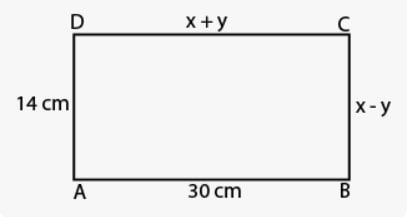
\includegraphics[width=\columnwidth]{figs/rectq8.jpg}
		\caption{rect ABCD}
		\label{fig:Fig1}
\end{figure}
	\section{Discrete}
	\item what is the HCF of smallest prime number and the smallest composite number?
	\item Given that $\sqrt{2}$ is irrational, prove that $\brak{5+3\sqrt2}$ is an irrational number.
	\item Find the sum of $8$ multiples of $3$.
	\item Find the HCF and LCM of $404$ and $96$ and verify that HCF*LCM = product of the given numbers.

			\item In an $AP$, if the common difference $(d) = -4$, and the seventh term$(a_7)$ is $4$, then find the first term.		
			\item The sum of four consecuive numbers in an AP is $32$ and the ratio of the product of the first and the last term to the product of two middle term is $7:15$. Find the numbers.

